\documentclass{article}
\usepackage{graphicx}

\begin{document}

\title{\textbf{Summary of Case Study: Crypto Arbitrage Opportunity Between Poloniex and Binance}}
\maketitle

\section{Problem}
\subsection{Intro}
This case study focuses on identifying and capitalizing on a crypto arbitrage opportunity between two exchanges, Poloniex and Binance. We will examine various currency pairs, including DOT/USDT, LTC/USDT, and TRX/USDT. The objective is to analyze indicators that signify arbitrage opportunities, determine their
duration, and understand the primary driving factors behind them. Additionally, we will explore how to
leverage illiquidity and strategically build positions on Poloniex for subsequent transfer to Binance. Finally,
we will consider the required inventory amount to break even on withdrawals.
\subsection{Data}
The data used in this case study is from the Poloniex and Binance exchanges in the form of tick-by-tick trades. The data was collected from a complete day of trading on August 15, 2022 for the DOT/USDT, LTC/USDT, and TRX/USDT currency pairs. These currency pairs were chosen because they are all traded on both exchanges and have a high trading volume. An additional reason for choosing these currency pairs is that they are all traded against USDT, which is a stablecoin that is pegged to the US dollar. This means that we can assume that the price of USDT is constant and that any price differences between the exchanges are due to arbitrage opportunities.

\newpage
\section{Analysis}
\subsection{Indicators}
In order to compare arbitrage opportunities accross exchanges we will need a time series of bid/ask data for both exchanges. What would be best is a dataset that contains all orderbook updates for both exchanges. With this we can compare the bid/ask prices of the two exchanges to determine if arbitrage opportunities are possible. We will also have to include trading fees associated with each exchange.
\subsection{Driving Factors}
\begin{itemize}
  \item Market Liquidity: Leads to pricing discrepancies
  \item Regulatory Differences: Different countries/jurisdictions may have different policies/restrictions that affects the pricing and availabilities for currencies and assets
  \item Geographical Factors: May leads to regulatory differences; also includes time zone differences for example, leading to price disparities during overlappign trading hours
  \item Technological Advancements: Technology often increases market efficiency and reduces arbitrage duration
  \item Market Inefficiencies: Arbitrage arises when where are some temporary discrepancies in pricing caused by market inefficiency
\end{itemize}
\subsection{Additional Exchanges}
\begin{itemize}
  \item Coinbase Pro, also known as GDAX (Global Digital Asset Exchange)
  \item Bitstamp
  \item KuCoin
  \item OKEx
\end{itemize}
\subsection{Illiquidity}
\begin{itemize}
  \item Order Book Depth: A deeper order book indicates a higher number of buy and sell orders at various price levels, which generally leads to better liquidity
  \item Trading Volume: Higher trading volumes suggest greater market activity and ease of executing trades
\end{itemize}

\section{Proposed Strategy}
Websocket stream bid and ask price data from Poloniex and Binance. Let $B_p$, $A_p$ denote the bid/ask prices on Poloniex and $B_b$, $A_b$ denote the bid/ask prices on Binance. Denote the trading fee cost in percent as the variable $F_P$, $F_B$ for Poloniex and Binance respectively. Denote $G$ to be the constant gas fees or on-chain transfer fees. If \[(A_p * F_P) + G < (B_b * (1 - F_B)),\] then go long on Poloniex and short on Binance. Transfer tokens from Poloniex to Binance (cost of G) to close out the short position. Profit per token will be \[[(B_b * (1 - FB))] - [(A_p * FP) + G].\] Make sure there is a margin of safety on the trade (i.e., only trade when ROI is greater than some predetermined number - this will account for adverse affects during the trade).

\begin{figure}
  \centering
  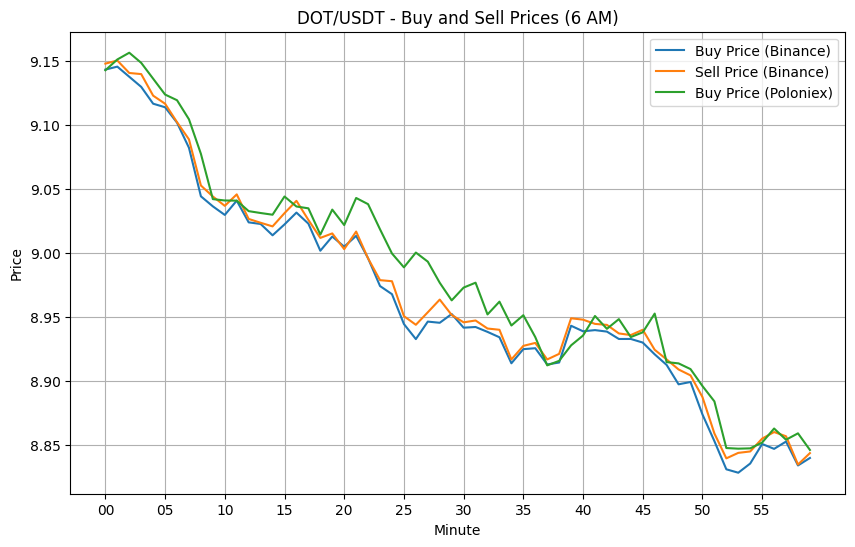
\includegraphics[width=\linewidth]{arbitrage.png}
  \caption{Comparison of bid/ask prices between Poloniex and Binance for the DOT/USDT currency pair.}
  \label{fig:arbitrage}
\end{figure}

\newpage
\section{Conclusion}
This case study aimed to identify and exploit crypto arbitrage opportunities between Poloniex and Binance. Through the analysis of indicators, such as price differentials, duration of opportunities, and driving factors, we can gain insights into the dynamics of arbitrage with crypto. We also explored how to leverage illiquidity and strategically build positions on Poloniex for subsequent transfer to Binance. Finally, we considered the required inventory amount to break even on withdrawals. Overall, we found that arbitrage opportunities are common and can be exploited with the right strategy. However, there are many risks involved, such as regulatory and technological factors, that can lead to losses. Therefore, it is important to be aware of these risks and to have a well thought out strategy before engaging in arbitrage.

\end{document}
